\chapter{Codierungstheorie}

\section{Grundbegriffe und einfache Beispiele}

\subsection{Codierung} (Kanalcodierung)\\
Sicherung von Daten/Nachrichten gegen zuf\"allig auftretenden Fehler bei Speicherung/\"Ubertragung.\\
\begin{figure}[h]
	\centering
	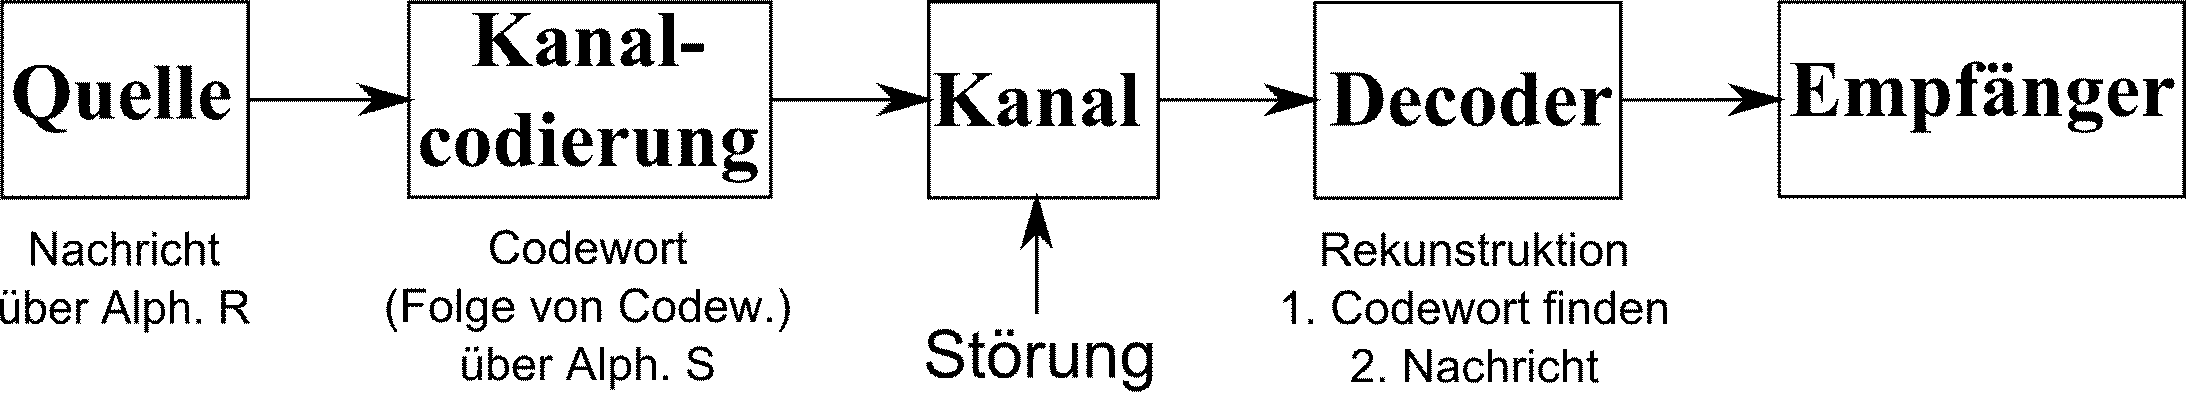
\includegraphics[width=15cm]{./img/codierung_schaubild.png}
	\caption{Schaubild der Codierung}
	\label{img:Schaubild Codierung}
\end{figure}

\subsection{Ziele}
\begin{itemize}
	\item M\"oglichst viele Fehler erkennen und gegebenenfalls korrigieren. %ABKUERZUNG
	\item Aufwand f\"ur Codierung und Decodierung m\"oglichst gering.
\end{itemize}

\section{Grundprinzip}
Hinzuf\"ugen von Redundanz
\\
Es gibt zwei Typen um Redundanz zu erzeugen.
\subsection{FEC-Verfahren (Forward Error Correction)}
Aufgetretene Fehler sollen erkannt \underline{und} korrigiert werden.\\
Vorteil: keine Verz\"ogerung der \"Ubertragung aber ggf. gro\ss e Redundanz notwendig.

\subsection{ARQ-Verfahren (Automatic Repeat Request)}
Aufgetretene Fehler sollen erkannt werden, werden nicht korrigiert. Stattdessen  wiederholt die \"Ubertragung beim Sender anfordern.\\
\\
Vorteil: geringe Redundanz, aber Verz\"ogerung.\\
\\
\subsubsection{Beispiele}
\subsection{Parity-Check-Codes}
z.B. Nachrichten: 00, 01, 10, 11\\
\\
Codierung:
\begin{align*}
	00 &\rightarrow 000\\
	01 &\rightarrow 011\\
	10 &\rightarrow 101\\
	11 &\rightarrow 110
\end{align*}
(gerade Anzahl von Einsen in den Codew\"ortern)\\
\\
1 Fehler wird erkannt, nicht korrigiert.\\
2 Fehler werden nicht erkannt.

\subsection{Wiederholungscode}
Nachrichten wie in 1.\\
\\
Codierung:
\begin{align*}
	00 &\rightarrow 000000\\
	01 &\rightarrow 010101\\
	10 &\rightarrow 101010\\
	11 &\rightarrow 111111
\end{align*}	
(3-Fache Wiederholung)\\
\\
1 Fehler wird erkannt und korrigiert.\\
\underline{01}01\underline{01} $\rightarrow$ 010101 $\rightarrow$ 01 \\
Nachrichten wie in 1.
Codierung:
\begin{align*}
	00 &\rightarrow 00000\\
	01 &\rightarrow 01101\\
	10 &\rightarrow 10110\\
	11 &\rightarrow 11011
\end{align*}
Je zwei Codew\"orter unterscheiden sich an mindestens 3 Positionen.\\
Angenommen 1 Fehler tritt bei \"Ubertragung auf. Dann gibt es genau ein Codewort, dass sich vom empfangenen Wort an genau einer Stelle unterscheidet; in das wird decodiert.

Muss immer Ungerade unterschiede in Codew\"ortern sein. Bei 5 diffs sind 2 Fehler korrigierbar.

\subsection{(ehmaliger) ISBN-Code}
International Standard Book Number\\
\\
10-Stelliger Code\\
Erste 9 Ziffern haben inhaltliche Bedingung ($\entspricht$ Nachricht)\\
10. Ziffer: Pr\"ufziffer\\
\\
Beispiel: 3-540-26121-? (Land - Verlag - Buchnummer - Pr\"ufziffer)\\
\\
Uncodierte W\"orter sind gebildet \"uber $R=\{0, \ldots, 9\}$\\
Codierte W\"orter sind gebildet \"uber $S=\{0, \ldots, 9, X\}$\\
\\
ISBN-Wort $C_{10}C_9\ldots C_2C_1$\\
$C_{10}\ldots C_2$ inhaltliche Bedingung, $C_1$ wird so gew\"ahlt, dass
\begin{align*}
	\sum^{10}_{k=1} k \cdot C_k &\equiv 0 (\md{11})\\
	10\cdot C_{10}+\ldots + 2\cdot C_2 + C_1 &\equiv 0(\md{11})
\end{align*}
falls $C_1 = 10$ so setzte $C_1 = X$\\
$C_1$ vom Beispiel ausrechnen.
\begin{align*}
	10\cdot 3+9\cdot 5+8\cdot 4+7\cdot 0+6\cdot 2+5\cdot 6+4\cdot 1+3\cdot 2+2\cdot 1+C_1 &\equiv 0 (\md{11})\\
	161 + C_1 &\equiv 0 (\md{11}) \Rightarrow C_1 = 4
\end{align*}
\"Andern einer Ziffer wird erkannt:\\
$C_{10} C_9\ldots C_2 C_1 \rightarrow\ C_i$ wird $X_i \neq C_i$ ersetzt\\
$C_{10} \ldots C_{i+1} X_i C_{i-1} \ldots C_1$
\[
	\sum^{10}_{k=1, k \neq i} k \cdot C_k + i \cdot x_i = 
	\underbrace{\sum^{10}_{k=1, k \neq i} k \cdot C_k}_{\equiv 0 (\md{11})}
	\overbrace{
			\underset{\underset{\nequiv 0 (\md{11})}{\uparrow}}{i} 
			\cdot (\underbrace{x_i-c_i}_{\nequiv 0 (\md{11})}) 
	}^{\nequiv 0 (\md{11})}
	\nequiv 0(\md{11})	
\]
Fehler wird erkannt, Korrektur nicht m\"oglich.\\
\\
$3-540-26121-4 \equiv 0(\md{11})$\\ \\
$\left.
\begin{matrix}
	3-540-26121-\mathbf{6} \\
	3-540-2612\mathbf{2}-4
\end{matrix}
\right\} \text{Pr\"ufsumme 2.}
$\\
Vertauschung von Zwei Ziffern wird erkannt.\\
$C_i$ und $C_j$ vertauscht.\\
O.B.d.A $C_i \neq C_j$\\
$C_{10} \ldots \underset{\stackrel{\uparrow}{i}}{C_j} \ldots \underset{\stackrel{\uparrow}{j}}{C_i} \ldots C_1$\\
\begin{align*}
	\sum^{10}_{k=1, k\neq i,j} k \cdot C_k + i \cdot 	C_j + j \cdot C_i
	&= \sum^{10}_{k=1} k \cdot C_k + i(C_j-C_i)+j(C_i-C_j)\\
	&= 
	\underbrace{\sum^{10}_{k=1} k \cdot C_k}_{\equiv 0 (\md{11})}
	 + 
	 \underbrace{(C_j-C_i)}_{\nequiv 0 (\md{11})}
	 \underbrace{(i-j)}_{\nequiv 0 (\md{11})}
	 \nequiv 0 (\md{11})
\end{align*}
Vertauschung wird durch gewichtete Quersummen erkannt.


\subsection{EAN-13-Code}
European Article Number\\
13-Stelliger Code, erste 12 Ziffer sind inhaltlich festgelegt.\\
13. Ziffer ist Pr\"ufziffer.\\
$R=S=\{ 0, \ldots, 9\}$ \\
$C_1 \ldots C_{12} C_{13}$\\
\\
$C_1 \ldots C_{12}$ inhaltliche Angabe (in der Regel):\\
$C_1 C_2$ Herstellerland (40-43 Deutschland)\\
$C_6 \ldots C_7$ Hersteller
$C_8 \ldots C_{12}$ interne Produktions Nummer\\
\\
$C_{13}$ so gew\"ahlt, dass
\[
	C_1 + 3\cdot C_2 + C_3 + 3\cdot C_4 + \ldots + 3\cdot C_{12} + C_{13} \equiv 0 (\md{10})
\]
$x \rightarrow 3x$ Permutation auf $\Z_{10} (\md{10})$, da $ggT(3,10)=1$, %FORMATTING vom ggT?
1 Fehler wird erkannt. Vertauschung in der Regel nicht erkannt. \\
\\
\"Ubersetzung in Barcode:
\[	
	C_1 C_2 \ldots C_7 C_8 \ldots C_{13}
\]
Jede der Ziffern $C_2, \ldots, C_{13}$ wird durch einen 0-1-String der L\"ange 7 bin\"ar codiert. \\
$0 \entspricht$ wei\ss er Balken, $1 \entspricht$ schwarzer Balken. \\
Codierung sorgt daf\"ur, dass nie mehr als 4 wei\ss e oder schwarze Balken nebeneinander stehen. \\
\begin{figure}[h]
	\centering
	
\includegraphics{./img/ean13.png}
	\caption{EAN-13 Barcode}
	\label{img:EAN-13 Barcode}
\end{figure}
\\
Schmalen Balken in Mitte und am Rand, sind nur Abtrennzeichen, die nichts mit EAN zu tun haben und nur beim einscannen helfen.\\
\[
	5 \text{ zu }0110001_2
\]
$C_2,\ldots, C_7$ werden nach Code A oder Code B codiert. $C_1$ bestimmt welcher dieser beiden Codes verwendet wird. \\
$C_8,\ldots, C_{13}$ werden nach Code C codiert.\\
$C_1$ ergibt sich aus der Art der Codierung von $C_2,\ldots,C_7$

\begin{center}
	\begin{tabular}{| c | c | c | c | p{2cm} |}
	\hline
	 &\multicolumn{2}{|c|}{\textbf{Ziffern $\mathbf{C_2 - C_7}$}} & \textbf{Ziffern $\mathbf{C_8 - C_{13}}$} & \textbf{bestimmt durch} $\mathbf{C_1}$ \\
	\hline
	\textbf{Zeichen} & \textbf{Code A} & \textbf{Code B} & \textbf{Code C} & \textbf{Code D}\\
	\hline
	\textbf{0} &	0001101 &	0100111 &	1110010 &	AAAAAA\\
	\textbf{1} &	0011001 &	0110011 &	1100110 &	AABABB\\
	\textbf{2} &	0010011 &	0011011 &	1101100 &	AABBAB\\
	\textbf{3} &	0111101 &	0100001 &	1000010 &	AABBBA\\
	\textbf{4} &	0100011 &	0011101 &	1011100 &	ABAABB\\
	\textbf{5} &	0110001 &	0111001 &	1001110 &	ABBAAB\\
	\textbf{6} &	0101111 &	0000101 &	1010000 &	ABBBAA\\
	\textbf{7} &	0111011 &	0010001 &	1000100 & 	ABABAB\\
	\textbf{8} &	0110111 &	0001001 &	1001000 &	ABABBA\\
	\textbf{9} &	0001011 &	0010111 &	1110100 &	ABBABA\\
	\hline
	\end{tabular}
\end{center}
Codew\"orter von Code A,B oder C kommen nur einmal vor. Daher treten nie mehr als 4 gleiche Balken nebeneinander auf. \\

\section{Blockcodes}
\begin{align*}
	00 \rightarrow & 00000\\
	01 \rightarrow & 01101\\
	10 \rightarrow & 10110\\
	11 \rightarrow & 11011
\end{align*}

\subsection{Definition}

$S$ endl. Menge (=Alphabet), $n \in \N$. \\
Ein Blockcode $\mathcal{C}$
der (Block-)L\"ange $n$ \"uber $S$ ist Teilmenge von $S^n=\underset{\longleftarrow \ \  n\ \  \longrightarrow}{S \times \ldots \times S}$ \\ % Pfeilspass <- n -> \times
\\
Elemente von $\mathcal{C}$ hei\ss en \textbf{Codew\"orter}. \\
Ist $\left| S \right| = 2$ (i.d.R. $S=\lbrace 0,1 \rbrace$, so \textbf{bin\"ar} Code.\\
$\left| \mathcal{C} \right| = m$, so ist $m \leq \left| S \right| ^ n$. \\
\\
Dann lassen sich $n$ Informationssymbole (oder Strings von Informationssymbolen) codieren (Codierungsfunktion). Folge von Informationssymbolen (oder Strings) werden dann in Folge von Codew\"ortern codiert.

\subsection{Definition: Hamming-Abstand}
$S$ endl. Alphabet, $n \in \N$. \\
$a,b \in S^n$ $a=(a_1, \ldots, a_n)$, $b=(b_1, \ldots, b_n)$ \\
$d(a, b)= \sharp \lbrace i : a_i \neq b_i \rbrace$ \\
\textbf{Hamming-Abstand} von $a$ und $b$ (Anzahl der unterschiedlichen Stellen). \\
(Richard W. Hamming, 1915-1998, Begr\"under der Codierungstheorie)

\subsubsection{Eigenschaften}
\begin{description}
	\item[a)] $d(a,b)=0 \Leftrightarrow a=b$
	\item[b)] $d(a,b)=d(b,a)$
	\item[c)] $d(a,b) \leq d(a,c) + d(c,b)$ (Dreiecksungleichung) \\
			($a_i \neq b_i \Rightarrow a_i \neq c_i$ oder $b_i \neq c_i$) 
	\item[d)] 	Wenn $(S,+)$ komm. Gruppe, dann auch $S^n$\\
				$[ (a_1,\ldots a_n) + (b_1, \ldots b_n) = (a_1+b_1,\ldots, a_n+b_n)]$\\
				$d(a,b)=d(a+c,b+c)$ (Translationsinvarianz)				
\end{description}

\noindent Also: Wird $x \in \mathcal{C}$ gesendet und $y \in S^n$ wird empfangen und $d(x,y)=k$, so sind $k$ Fehler aufgetreten.
\subsection{Definition}
\subsubsection{a) Hamming-Decodierung}
f\"ur Blockcode $\mathcal{C} \subseteq$ $S^n$ \\
Wird $y \in S^n$ empfangen, so wird $y$ zu einem Codewort $x' \in \mathcal{C}$ decodiert, das unter allen Codew\"ortern minimalen Hamming-Abstand zu $y$ hat.
\[
	d(x',y)=min\  d(x,y), x \in \mathcal{C}
\]
($x'$ muss nicht eindeutig bestimmt sein)\\
z.B. $\mathcal{C}$ $ = \{ (0000), (1111) \}$\\
Empfangen: $0011$ $x'$ nicht eindeutig in diesem Fall.\\
\\
($\left| S \right | = 2$: Hamming-Decodierung ist bestm\"oglich, falls jedes Symbol in einem Codewort mit der gleichen Wahrscheinlichkeit $p < \frac{1}{2}$ ver\"andert wird und wenn jedes Codewort gleich wahrscheinlich ist.)

\subsubsection{b) Minimalabstand}
$\mathcal{C}$ Blockcode in $S^n$, Minimalabstand von $\mathcal{C}$:
\[
	d(\mathcal{C}) = min \  d(x,x')\mathbf{,}\ \  x,x' \in \mathcal{C}, x \neq x'
\]
(Ist $\left| \mathcal{C} \right| = 1$, so $d(\mathcal{C})=n$)\\
$[Bsp: \mathcal{C} = \lbrace (00000),(01101),(10110),(11011) \rbrace , d(\mathcal{C})=3]$

\subsubsection{c)} 
Ein Blockcode $\mathcal{C}$ ist \textbf{t-Felder-korrigierend}, falls $d(\mathcal{C}) \geq 2t+1$, und er hei\ss t \textbf{t-Fehler-erkennend}, falls $d(\mathcal{C}) \geq t+1$. \\
\\
Begr\"undung f\"ur die Bezeichnung in c) \\
"`Kugel"' vom Radius $t$ um $x \in \mathcal{C}: K_t(x) = \{y \in S^n: d(x,y) \leq t\}$\\
\\
Ist $d(\mathcal{C}) \geq 2t+1$, so sind Kugelm vom Radius $t$ um Codew\"orter disjunkt. \\
\\
Angenommen es existiert $y \in S^n$ mit $y \in K_t(x)\cap K_t(x')$, $x,x' \in \mathcal{C}, x \neq x'$. Dann $d(x,x') \leq d(x,y)+d(y,x') \leq t+t = 2t$. Widerspruch\\ %LIGHTNING ARROW \lightning
$x \in \mathcal{C}$ gesendet, $y$ wird empfangen, und angenommen maximal $t$-Fehler sind aufgetreten, dann $y \in K_t(x)$ und Abstand zu jedem anderem Codewort ist $> t$\\
$\Rightarrow$ Hamming-Decodierung ist korrekt.\\
$d(\mathcal{C}) \geq t+1$ und es treten maximal $t$ minimal $1$ Fehler auf, so ist $y$ kein Codewort.\\
\\
\textbf{Bsp}: 
\begin{description}
	\item[a)] $n$-fach Wiederholungscode \\
	$
	\begin{matrix} 
		S_n & \rightarrow & \underset{\longleftarrow \ \ n \ \ \longrightarrow}{S_1 S_1 \ldots S_1} \\ 
		\vdots \\
		S_k & \rightarrow & \underset{\longleftarrow \ \ n \ \ \longrightarrow}{S_k S_k \ldots S_k}
	\end{matrix}$\\
	\\
	$\mathcal{C}=\lbrace (s,s,\ldots,s): s \in S \rbrace \subseteq S^n$ \\
	$d(\mathcal{C})=n$ \\
	\\
	$\left\lfloor \frac{n-1}{2} \right\rfloor$-Fehler-korr.
	\item[b)] ISBN, EAN-Codes, $d(\mathcal{C})=2$, 1-Fehler-erkennend.
\end{description}

%Verbesser + Verschoenert, aber kein plan was der titel hier ist
\section{Titel???}

$d(\mathcal{C}) \geq 2 \cdot t + 1,\ \mathcal{C} \subseteq R^N$ \\
$K_t(x) \cap K_t(x')=\emptyset$ \\
$x, x' \in \mathcal{C},\ x \neq x'$ \\
\\
$y$ empfangen:
\begin{itemize}
\item falls $y$ in $K_t(x)$ liegt f\"ur einen $x \in \mathcal{C}$, so wird $y$ nach $x$ decodiert (Korrekt, falls max. $t$ Fehler aufgetreten sind)
\item  falls $y$ in keiner $K_t(x)$ liegt, so kann es mehrere Codew\"orter geben mit gleichem min. Abstand zu $y$. (Dann keine eindeutige  Decodierung)
\end{itemize}

\subsection{Definition: Perfekter Code}
Code $\mathcal{C} \subseteq R^n$ hei\ss t perfekt, falls es ein $t \in \N_0$ gibt, mit der Eigenschaft:
\[
	R^n = \bigcup_{x \in \mathcal{C}} K_t(x) \quad \text{und} \quad K_t(x) \cap K_t(x') = \emptyset \quad \text{f\"ur}\quad x,x' \in \mathcal{C},\ x \neq x'
\]
Dann ist $d(\mathcal{C})=2 \cdot t + 1$, falls $\left| \mathcal{C} \right| > 1$: \\
Ang. $d(\mathcal{C}) \leq 2\cdot t$. W\"ahle $x,x' \in \mathcal{C},\ x \neq x'$, mit $d(x,x') = d(\mathcal{C}) \leq 2 \cdot t$. \\
W\"ahle $y \in R^n$ mit $d(x,y)=t,\ d(y,x') \leq t$\\
$y \in K_t(x) \cap K_t(x')$ Widerspruch\\
$d(\mathcal{C}) \leq 2 \cdot t + 1$ \\
\\
W\"ahle $x \in \mathcal{C}$, w\"ahle $y \in R^n$ mit $d(x,y)=t+1$. Nach Vorraussetzung existiert $x' \in \mathcal{C}$ mit $y \in K_t(x')$. 
\begin{align*}
	&d(x,x') \leq d(x,y) + d(y,x') \leq t+1+t = 2 \cdot t + 1 \\
	&d(\mathcal{C}) \leq 2\cdot t + 1
\end{align*}	

\subsection{Gibt es perfekte Codes?}
Trivial Beispiele:
\begin{itemize}
	\item einelementige Codes (t=n)
	\item $\mathcal{C} = R^n$ (t=0) \\
				(Jedes Element ist ein Codewort)
	\item $n$-fache Wiederholungscode \"uber $Z_2$ \\
				$n=2 \cdot t +1$ \\
				$\mathcal{C} = \lbrace \underset{\longleftarrow n \longrightarrow}{(0,\ldots,0)},\underset{\longleftarrow n \longrightarrow}{(1,\ldots,1)}\rbrace$
\end{itemize}

\subsection{Lemma}
$\left| R \right| = q,\ x \in R^n,\ t \in \N$ \\
Dann ist $\left| K_t(x) \right| = \sum_{i=0}^t \binom{n}{i} \cdot (q-1)^i$ \\
$\left(\binom{n}{i}=\frac{n\!}{i\! \cdot (n-i)\!}\right)$

\subsubsection{Beweis}
Abstand 0 zu $x$: 1 Word (n\"amlich $x$): $\binom{n}{0} \cdot (q-1)^0 =1$ \\
Abstand $i>0$ zu x: \\
Anzahl der Auswahl von $i$ Positionen aus $n$ Positionen: $\binom{n}{i}$ \\
An jeder Position $q-1$ \"Anderungsm\"oglichkeiten. \\
$\rightarrow$ insgesamt $(q-1)^i$ M\"oglichkeiten, \\
Anzahl der W\"orter vom Abstand $i$ von $x$: $\binom{n}{i} \cdot (q-1)^i$

\subsubsection{Satz}
Sei $\mathcal{C}$ ein Code der L\"ange $n$ \"uber $R$, $\left| \mathcal{C} \right|> 1, \left|R\right| = q$. Sei $t \in \N_0$ maximal mit $d(\mathcal{C}) \geq 2 \cdot t + 1,\ t=\lfloor \frac{d(\mathcal{C})-1}{2}\rfloor$.
\begin{itemize}
	\item[a)] (Kugelpackungsschranke) \\
	$\left|\mathcal{C}\right| \leq \frac{q^n}{\sum_{i=0}^t \binom{n}{i} \cdot (q-1)^i}$
	\item[b)] $\mathcal{C}$ ist perfekt $\Leftrightarrow$ in a) gilt Gleichheit, d.h. \\
	$\left|\mathcal{C}\right| = \frac{q^n}{\sum_{i=0}^t \binom{n}{i} \cdot (q-1)^i}$
\end{itemize}

\subsubsection{Beweis}
a)
\begin{align*}
	&d(\mathcal{C}) \geq 2 \cdot t + 1,\text{ daher }K_t(x) \cap K_t(x')=\emptyset,\ x\neq x',\ x,x' \in \mathcal{C}  \\
	&R^n \geq \underset{x \in \mathcal{C}}{\bigcup} K_t(x) \\
	&q^n=\left|R^n\right| \\
	&\left| \bigcup_{x \in \mathcal{C}} K_t(x) \right| = \sum_{x \in \mathcal{C}} \left| K_t(x) \right|
	\underset{Lemma}{=}\left| \mathcal{C} \right| \cdot \sum_{i=0}^t \binom{n}{i} \cdot (q-1)^i\\
\end{align*}
b)
\begin{align*}
	&\Rightarrow:d(\mathcal{C})=2 \cdot t +1 \\
	&R^n = \bigcup_{x \in \mathcal{C}} K_t(x) \Rightarrow \text{Gleichheit in a)}\\
	&\Leftarrow: \text{Gleichheit} \Rightarrow R^n=\bigcup K_t(x) \Rightarrow \mathcal{C} \text{ perfekt.}
\end{align*}

%Teil 2 der Vorlesung
\subsection{Bsp: Bin\"arer Hamming-Code der L\"ange 7}

$R=\Z_2=\lbrace 0,1 \rbrace$ $\mathcal{C}$ perfekt, $d(\mathcal{C})=3,\ \left| \mathcal{C} \right| = 16$ \\
1-Fehler-Korrigierend
\begin{align*}
\mathcal{C} = \lbrace (C_1,\ldots,C_7) : C_i \in \Z_2,\ &C_1 + C_4 + C_6 + C_7 = 0,\\
										&C_2 + C_4 + C_5 + C_7 = 0,\\
										&C_3 + C_5 + C_6 + C_7 = 0\\
										 &\rbrace \subseteq \Z_2^7
\end{align*}
$\mathcal{C}$ ist Unterraum von $\Z_2^7$ \\
$(C_1,\ldots,C_7) \in \mathcal{C},\ (C_1',\ldots,C_7') \in \mathcal{C}$ \\
$(C_1 + C_1',\ldots,C_7+C_7')\ \ (C_1+C_1') + (C_4+C_4') + (C_6+C_6') + (C_7+C_7') = 0$ \\
$dim(\mathcal{C})=4,\ C_4,C_5,C_6,C_7$ frei w\"ahlbar $\curvearrowright C_1,C_2,C_3$ festgelegt \\
Basis:
\begin{align*}
	&(\ldots 1000) \rightarrow (1101000) \\
	&(\ldots 0100) \rightarrow (0110100) \quad \left| \mathcal{C} \right| =2^4 =16\\
	&(\ldots 0010) \rightarrow (1010010) \\
	&(\ldots 0001) \rightarrow (1110001)
\end{align*}
$d(\mathcal{C})=3:$\\
Ang. $d(\mathcal{C})=d$. W\"ahle $x,x' \in \mathcal{C}$ mit $d(x,x')=d$\\
Translationsinvarianz der Metrik: \\
\begin{align*}
	d &=d(x,x')=d(x+x,x+x')=d(0,x+x') \\
	wt(x) &= \text{ Anzahl der Einsen in } x \\
	&= d(0,x)\\
	d(\mathcal{C}) &= \min wt(x),\quad x \in \mathcal{C},\quad x \neq \mathcal{V}
\end{align*}
Zeige: Jeder Vektor $\neq v$ in $\mathcal{C}$ enth\"alt mind. 3 Einsen.\\
$= 3$ weist man nach durch \"uberpr\"ufen aller 15 von $\mathcal{V}$ verschiedenen Codew\"ortern oder durch Analyse der Gleichung. 
\begin{align*}
	&(C_1,\ldots,C_7) \in \mathcal{C} \text{ Ang. } C_7=1 \\
	\Rightarrow &C_1+C_4+C_6=1. \text{ Wenn alle Eins } \checked \\
	&C_1=1,C_4=C_6=0\\
	&C_4=1,C_1=C_6=0\\
	&C_6=1,C_1=C_4=0\\
	&C_1, C_2\text{ oder } C_3 = 1
\end{align*}
2. Fall: $C_7=1,C_4=1,C_1=0,C_2 \text{ oder } C_3=1$ \\
3. Fall: analog zu Fall 2.\\
1. Fall: $C_1=1,C_4=C_6=0, C_7=1$, o.B.d.A. $C_2=C_3=0 \Rightarrow C_5=1$\\
$d(\mathcal{C}) \leq 3,\ d(\mathcal{C})=3=2 \cdot 1 + 1$\\
\\
Pr\"ufe nach, ob bei Kugelpackungsschranke Gleichheit gilt:
\begin{align*}
	\left|\mathcal{C}\right| &=16\\
	\left|\mathcal{C}\right| &\leq \frac{q^n}{\sum_{i=0}^t \binom{n}{i} \cdot (q-1)^i} \quad (q=2, t=1, n=7)\\
	&=\frac{2^7}{1+\binom{7}{1}}=\frac{2^7}{2^3}=2^4=16\\
	&\mathcal{C}\text{ perfekt!}
\end{align*}

% Vorlesung vom 28.01.2010
\section{Lineare Codes}
\subsection{Definition: linearer Code}
Sei $K$ ein endlicher K\"orper, $n \in \N$. Ein linearer Code $\mathcal{C}$ der L\"ange $n$ ist ein Unterraum von $K^n$. (Zeilenvektoren) [Alphabet = $k$] \\
\\
Ist $dim(\mathcal{C})=k$, so hei\ss t $\mathcal{C}$ $\left[n,k\right]$-Code.\\
Ist $d(\mathcal{C})=d$, so $\left[ n,k,d \right]$-Code. \\
\\
Beachte: $\left| K \right| = q \Rightarrow \left| \mathcal{C} \right| =q^k$.\\
\subsection{Definition: Informationsrate}
Informationsrate (Rate) von $\mathcal{C}: \frac{k}{n}$.\\
\subsection{Bemerkung \"uber endliche K\"orper}
\begin{itemize}
	\item[a)] $p$ Primzahl, $\Z_p$ ist K\"orper der Ordnung $p$
	\item[b)] $K$ endlicher K\"orper $\Rightarrow \left| K \right| = p^m$, $p$ Primzahl, $m \in \N$.
	\item[c)] Zu jeder Primzahlpotenz $p^m$ existiert (bis auf Isomorphie) genau ein K\"orper der Ordnung $p^m$.
	\item[d)] $f$ sei irreduzibles Polynom vom Grad $m$ \"uber $\Z_p$.\\
	 $K=\lbrace g \in \Z_p [x] : Grad(g) \leq m-1 \rbrace, \quad \left| K \right| = p^m$\\
	$K$ wird K\"orper:\\
	Addition = \"ubliche Addition von Polynomen \\
	Multiplikation = normale Multiplikation + Reduktion $\md{f}$ \\
	(AES : $\left| K \right| = 2^8$)
\end{itemize}

\subsection{Bsp}
\begin{itemize}
	\item[a)] $n$-facher Wiederholungscode \"uber $\Z_p$\\
	$\mathcal{C}=\lbrace \underset{\longleftarrow n \longrightarrow}{(0,\ldots,0)},(1,\ldots,1),\ldots,(p-1,\ldots,p-1)\rbrace$\\
	$\mathcal{C}$ ist linerer Code, $\mathcal{C}=<(1,\ldots,1)>$\\
	$[n,1,n]$-Code
	\item[b)] Hamming-Code ist linearer [7,4,3]-Code \"uber $\Z_2$
	\item[c)] $\mathcal{C} = \lbrace (c_1,\ldots,c_n) : c_i \in \Z_p,\sum^n_{i=1}{c_i}=0 \rbrace$ \\
	$(p=2 : \text{ Parity Check Code})$, linear $[n,n-1,2]$-Code \"uber $\Z_p$\\
	Basis von $\mathcal{C}:(1,0,\ldots,0,p-1), (0,1,0,\ldots,0,p-1), \ldots, (0,\ldots,0,1,p-1)$
\end{itemize}
\subsection{Definition: Gewicht und Minimalgewicht}
$K$ endl. K\"orper
\begin{itemize}
	\item[a)] $x \in K^n$, so Gewicht von $x$, $wt(x)$, definiert durch $wt(x)=\sharp \lbrace i:x_i\neq0 \rbrace$
	\item[b)] $\lbrace 0 \rbrace \neq \mathcal{C} \subseteq K^n$, so ist das Minimalgewicht von $\mathcal{C}$ definiert durch $wt(\mathcal{C})=\underset{x\in\mathcal{C}, x\neq 0}{min} wt(x)$
\end{itemize}

\subsection{Satz}
Ist $\mathcal{C} \neq \lbrace 0 \rbrace$ ein linearer Code, so ist $d(\mathcal{C})=wt(\mathcal{C})$. (Beweis wie beim [7,4,3]-Hamming Code)

\subsection{Definition: Erzeugermatrix} %Nochmal im Vid anschauen....bin mir nicht sicher ob das hier stimmt.
Sei $\mathcal{C}$ ein $[n,k]$-Code \"uber $K$, sei $g_1=(g_{11},\ldots,g_{1n}),\ldots,(g_{k1},\ldots,g_{kn})=(g_{k1},\ldots,g_{kn})$ eine Basis von $\mathcal{C}$.
\[
\text{Dann hei\ss t die } k\times n\text{ -Matix } G=
\begin{pmatrix}
g_1\\
\vdots \\
g_k\\
\end{pmatrix}
=
\begin{pmatrix}
	g_{11}&\ldots&g_{1n}\\
	\vdots&&\vdots\\
	g_{k1}&\ldots&g_{kn}
\end{pmatrix}
\text{ Erzeugermatrix von } \mathcal{C}
\]
\subsection{Satz}
Sei $G$ ein Erzeugermatrix von $\mathcal{C}$.\\
Dann ist $\mathcal{C} = \lbrace \underset{1\times k}{u} \cdot \underset{k\times x}{G}: u \in K^k \rbrace$\\
Beweis:\\
$u=(u_1,\ldots,u_k),u_i\in K$\\
$uG=(u_1,\ldots,u_k) \cdot (g_1,\ldots,g_k)^t=u_1g_1+\ldots + u_kg_k \in \mathcal{C}$\\
\subsection{Bemerkung}
\begin{itemize}
	\item[a)] Die Abb 
	$\begin{cases}
		K^k & \rightarrow \mathcal{C}\\
		u & \mapsto uG
	\end{cases}$ ist bijektiv. \\
	$u \in K^k$ Informationsw\"orter \\
	Codert in Codew\"orter durch $uG$.
	\item[b)] Elementare Zeilenumformungen an Erzeugermatrix liefern Erzeugermatrix.
\end{itemize}
\subsection{Beispiel: Hamming-$[7,4]$-Code \"uber $\Z_7$}

\begin{align*}
\mathcal{C} = \lbrace (C_1,\ldots,C_7) : C_i \in \Z_2,\ &C_1 + C_4 + C_6 + C_7 = 0,\\
										&C_2 + C_4 + C_5 + C_7 = 0,\\
										&C_3 + C_5 + C_6 + C_7 = 0\\
										 &\rbrace \subseteq \Z_2^7
\end{align*}
\noindent
Erzeugermatrix:
\[	G=
	\begin{pmatrix}
		1 & 0 & 0 & 0 & 1 & 0 & 1\\
		0 & 1 & 0 & 0 & 0 & 1 & 1\\
		0 & 0 & 1 & 0 & 1 & 1 & 1\\
		0 & 0 & 0 & 1 & 1 & 1 & 0
	\end{pmatrix}
\]
Cod. eines Informationswort $(u_1,u_2,u_3,u_4)$ mit $G$
\[
	(u_1,u_2,u_3,u_4) \rightarrow (u_1,u_2,u_3,u_4) \cdot G =  (\mathbf{u_1,u_2,u_3,u_4},u_1+u_3+u_4,u_2+u_3+u_4,u_1+u_2+u_3)
\]
\subsection{Definition: Standardform}
$\mathcal{C} \  [n,k]$-Code Erzeugermatix $\mathcal{C}$ ist in Standardform, falls sie folgende Gestalt hat.
\begin{align*}
	G= \quad
	k
	\underset{\leftarrow \quad k \quad \rightarrow \quad \leftarrow (n-k) \rightarrow}{
	\begin{cases}
	\begin{pmatrix}
		1 & & 0\\
		 & \ddots & & & * & \\
		0 & & 1 & &
	\end{pmatrix}
	\end{cases}
	}
\end{align*}

Cod. $(u_1,\ldots,u_k) \cdot G = (u_1,\ldots,u_k,*,\ldots,*)$

\subsection{Satz}
Sei $\mathcal{C}$ ein $[n,k]$-Code \"uber $K$. Dann existiert $(n-k)\times n$-Matrix $H$ \"uber $K$ mit folgenden Eigenschaften: \\
Sei $y\in K^n$. Dann: $y \in \mathcal{C} \Leftrightarrow H \cdot y^t = \vec{0}$ 
\\
$H$ hei\ss t Kontrollmatrix von $\mathcal{C}$ ($\Leftrightarrow y \cdot H^t = \vec{0}$) \\
Es ist $rg(H)=n-k$ (Dann ist $H \cdot G^t=0$)

\subsection{Beweis}
Sei $g_1,\ldots,g_k$ Basis von $\mathcal{C}$, $G=
\begin{pmatrix}
g_1 \\
\vdots \\
g_2
\end{pmatrix} $ \\
$g_i=(g_{i1},\ldots,g_{in})$\\
Betrachte LGS: 
\begin{align*}
	g_{11} x_1 + \ldots + g_{1n} x_n &= 0\\
	\vdots&\\
	g_{k1} x_1 + \ldots + g_{kn} x_n &= 0
\end{align*}
d.h. $G \cdot
\begin{pmatrix}
x_1 \\
\vdots \\
x_n
\end{pmatrix}
= 0$. Koeffizientmatrix $G$ hat Rang $k$.\\
Dimension des L\"oungsraums dieses LGS $= n - k$ \\
Sei $h_1,\ldots,h_{n-k} \in K^n$ Basis des L\"osungsraums dieses LGS. \\
\[
	H=
	\begin{pmatrix}
	m\\
	\vdots \\
	h_{n-k}
	\end{pmatrix}
	, \quad H \cdot g^t_i =
	\begin{pmatrix}
	h_1 g_i^t \\
	\vdots \\
	h_{n-k} g_i^t
	\end{pmatrix}
	 =0,i=1,\ldots,k
\]
$H y^t=0$ f\"ur alle $y \in \mathcal{C}$.\\
$rg(H)=n-k \Rightarrow dim\ Kern(H) = k = dim ( \mathcal{C})$\\
$\mathcal{C}=Kern(H)$

\subsection{Bermerkung}
\begin{itemize}
	\item Kontrollmatrix kann zur Fehlererkennung verwendet werden.	
	\item Beweis liefert Verfahren: Erzeugermatrix $\rightarrow$ Kontrollmatrix
	\item Umgekehrt: Kontrollmatrix $\rightarrow$ Erzeugermatrix (Bilde Basis des L\"osungsraums von $H y^t=0)$
\end{itemize}

\subsection{Beispiel}
\begin{itemize}
	\item [a)] Parity-Check-Code \"uber $\Z_p$ \\
	$\mathcal{C} = \lbrace (c_1,\ldots,c_n): \sum^n_{i=1}{c_i}=0 \rbrace$\\ %,\quad k=n-1$\\ wo kam das hier her?
	$H=(1,1,\ldots,1)$\\
	$H \cdot
	\begin{pmatrix}
	c_1 \\
	\vdots \\
	c_n
	\end{pmatrix}
	= 0 \Leftrightarrow c_1 + \ldots c_n = 0 \Leftrightarrow (c_1,\ldots,c_n) \in \mathcal{C}$
	\item [b)] $[7,4]$-Hamming-Code
	\begin{align*}
	\mathcal{C} = \lbrace (C_1,\ldots,C_7) : C_i \in \Z_2,\ &C_1 + C_4 + C_6 + C_7 = 0,\\
										&C_2 + C_4 + C_5 + C_7 = 0,\\
										&C_3 + C_5 + C_6 + C_7 = 0\\
										 &\rbrace \subseteq \Z_2^7
	\end{align*}
	\[	H=
		\begin{pmatrix}
			1 & 0 & 0 & 1 & 0 & 1 & 1\\
			0 & 1 & 0 & 1 & 1 & 0 & 1\\
			0 & 0 & 1 & 0 & 1 & 1 & 1
		\end{pmatrix}
	\]
	\item [c)] $\mathcal{C}$ Code mit Erzeugermatrix\\
	$
	\begin{pmatrix}
		1 & 1 & 0 & 1\\
		0 & 1 & 0 & 1
	\end{pmatrix}$
	 $[4,2]$-Code \"uber $\Z_2$\\
	 $G \cdot
	 \begin{pmatrix}
	 x_1 \\
	 \vdots \\
	 x_4
	 \end{pmatrix}
	 =0$
	 \begin{align*}
	 	x_1+&x_2 + x_4=0\\
	 	&x_2 + x_4 =0
	\end{align*}
	$x_5,x_4$ frei w\"ahlen, $x_1,x_2$ fesgelegt.\\
	\[
		\text{Basis }
		(0 0 1 0), (0 1 0 1)
	\]	
	\[
		\text{Kontrollmatrix }
		H=
		\begin{pmatrix}
			0 & 0 & 1 & 0 \\
			0 & 1 & 0 & 1
		\end{pmatrix}
	\]
	$\mathcal{C} \lbrace (c_1,\ldots,c_4) : c_3=0,c_2+c_4=0\rbrace$	
\end{itemize}

%
%	Vorlesung vom 04.02.2010
%
\subsection{Satz}
$\mathcal{C}$ $[n,k]$-Code, $\mathcal{C} \neq \lbrace \vec{0} \rbrace, K^n$, Kontrollmatrix $H$.\\
\begin{align*}
d(\mathcal{C})=wt(\mathcal{C}) &= min \quad 	\lbrace r : \text{ in H gibt es r linear abh\"anige Spalten}  \rbrace \\
&= max  \quad \lbrace r : \text{ je r-1 Spalten linear unabh\"angig} \rbrace
\end{align*}

\subsubsection{Beweis}
$s_1,\ldots,s_n$ Spalten von $H$, L\"ange $n-k$. \\
$\mathcal{C} \neq \lbrace \vec{0} \rbrace, k \geq	 1, n-k<n \Rightarrow s_1,\ldots,s_n$ lin. abh\"angig.\\
Sei $min \lbrace r: \ldots \rbrace = w$. $s_{i_1},\ldots, s_{i_w}$ lin. abh\"angig. \\
Existiert $c_{i_1},\ldots,c_{i_w} \in K$, nicht alle $=0$, $c_{i_1} s_{i_1}+\ldots+ c_{i_w} s_{i_w}=0$ \\
$w \quad min \Rightarrow$ alle $c_{i_1},\ldots, c_{i_w} \neq 0$. \\
Def. $c=(c_1, \ldots,  c_n)$ mit den $c_{i_j}$ an den Stellen $i_j$, \"ubrige $c_i=0$
\begin{align*}
	\sum^n_{i=1}{c_i s_i} = c_{i_1} s_{i_1} + \ldots + c_{i_w} s_{i_w} &=0\\
	\sum^n_{i=1}{c_i s_i^t}&=0 \\
	Hc^t=0 \quad c \in \mathcal{C}
\end{align*}
$wt(c)=w$, Min. Gewicht von $\mathcal{C} \leq wt(c)=w$ \\
Ang. es ex. $0 \neq c' \in \mathcal{C}, wt(c')=w' < w$. $Hc'^t=0$\\
$c'=(c'_1, \ldots,  c'_n)$ \quad $\sum{c'_i s_i}^n_{i=1}=0 \Rightarrow$ $w'$ der Spalten $c_1,\ldots,c_n$ sind linear abh\"anging. Widerspruch! \\
$wt(c)=w$

%
% Stuff     <- What stuff? Hab hier nichts zwischen den beiden
%

\subsection{Beispiel: $[7,4]$-Hamming-Code \"uber $\Z_2$}
$H =
\begin{pmatrix}
1 & & 0 & 1 & 0 & 1\\
   &\ddots &    & 0 & 1 & 1\\
0 & & 1 & 1 & 1 & 1\\
\end{pmatrix}$ Kontrollmatrix.\\
Keine Spalte ist Nullspalte, keine zwei Spalten sind  gleich. 1.,2.,4. Spalte sind linear abh\"anging.
\[
	\begin{pmatrix}
	1\\
	0\\
	0\\
	\end{pmatrix} +
	\begin{pmatrix}
	0\\
	1\\
	0\\
	\end{pmatrix} +
	\begin{pmatrix}
	1\\
	1\\
	0\\
	\end{pmatrix} =
	\begin{pmatrix}
	0\\
	0\\
	0\\
	\end{pmatrix} \quad d(\mathcal{C})=3
\]
\subsection{Korollar: (Singleton-Schranke)}
Ist $\mathcal{C}$ ein linearer $[n,k]$-Code, $d(\mathcal{C})=d$, so gilt:
\[
	d \leq n-k + 1
\]
\subsubsection{Beweis}
2. Gleichheit: $d \leq rg(H)+1=n-k+1$ (Zeilen von H sind lin. unabh\"angig)
\subsection{Bemerkung: (Nebenklassen von Unterr\"aumen in Vektorr\"aumen)}
$\mathcal{C}$ ein Umterraum von Vektorraum $V$. F\"ur jedes $v \in V$:
\[
	v + \mathcal{C} = \lbrace v+x : x \in \mathcal{C} \rbrace
\]
\textbf{Nebenklasse} von $\mathcal{C}$ zu $v$.
\begin{itemize}
	\item[a)] $v_1,v_2 \in V$. Dann: \\
					$v_1 + \mathcal{C} = v_2 + \mathcal{C}$ oder $(v_1 + \mathcal{C}) \cap (v_2 + \mathcal{C}) = \emptyset$
	\item[b)] $v_1 + \mathcal{C} = v_2 + \mathcal{C} \Leftrightarrow v_1-v_2 \in \mathcal{C}$\\
						($v+ \mathcal{C} = \mathcal{C} (=\vec{0}+\mathcal{C}) \Leftrightarrow v \in \mathcal{C}$)
	\item[c)] W\"ahle aus jeder Nebenklasse einen Vektor $v_i$:\\
	\[
			V=\bigcup^{\bullet} (v_i + \mathcal{C})
	\]
	\item[d)] V Vektorraum \"uber endl. K\"orper: $\left| v + \mathcal{C} \right| = \left| \mathcal{C} \right|$
	\item[e)] $\mathcal{C}$ $[n,k]$-Code ($V=K^n, dim(\mathcal{C})=k,\left|\mathcal{C}\right|=q^k, \text{ falls } \left|K\right|=q$) \\
						Anzahl der Nebenklassen ist $q^{n-k}$
\end{itemize}

\section{Syndrom-Decodierung linearer Code}
$\mathcal{C}$ $[n,k]$-Code \"uber $K$, $\left| K \right| = q$, Kontrollmatrix $H$, $(n-k) \times n$-Matrix.\\
Ist $y \in K^n$, so hei\ss t $Hy^t \in K^{n-k}$ \textbf{Syndrom} von $y$.
\begin{itemize}
	\item[a)]	$x \in \mathcal{C} \Leftrightarrow Hx^t = 0$ ($x$ hat Syndrom $0$)
	\item[b)] $y_1,y_2 \in K^n$. $y_1,y_2$ liegen in der gleichen Nebenklasse zu $\mathcal{C}$ (d.h. $y_1 + \mathcal{C} = y_2 + \mathcal{C})\\ \Leftrightarrow y_1,y_2$ haben gleiches Syndrom \\
	(d.h. $Hy_1^t = Hy_2^t$)
	\[
		[y_1 + \mathcal{C} = y_2 + \mathcal{C} \Leftrightarrow y_1 - y_2 \in \mathcal{C} \Leftrightarrow 0 = H(y_1 - y_2)^t = Hy_1^t - Hy_2^t \Leftrightarrow Hy_1^t = Hy_2^t]
	\]
	\item[c)] Jedes $z \in K^{n-k}$ tritt als Syndrom auf.	 
\end{itemize}
Ang. $x \in \mathcal{C}$ wird gesendet, $y=x+f$, wird empfangen.\\
$f$ "Fehlervektor".\\
$y + \mathcal{C} = f + \mathcal{C}$, $y$ und $f$ haben das gleiche Syndrom, n\"amlich $Hy^t$.\\
Bestimmt in der Nebenklasse von $y$ ein $e$ mit kleinstm\"ogliche Gewicht (\textbf{Nebenklassenf\"uhrer}) \\
Decodierung: $y \rightarrow y - e \in \mathcal{C}$ (Hamming-Decodierung)\\
\\
Ordne die Nebenklassenf\"uhrer nach der lexikogr. ihrer Syndome. \\
Speicherbedarf: $q^{n-k}$ Nebenklassenf\"uhrer, jeder hat L\"ange $n$ \\
(Besser als Durchforsten der Liste aller Codew\"orter ($q^k$), falls $k \geq \frac{n}{2}$)\\
$\mathcal{C}$ $[70,50]$-Code \"uber $\Z_2$. $2^{20}$ Nebenklassenf\"uhrer, je $70$ BitL\"ange.\\
Speicher: $70 \cdot 2^{20} Bit \approx 8,75 \text{ MegaByte}$ \\
Speicher f\"ur Codew\"orter: $70 \cdot 2^{50} \text{ Bit} = 9 \text{ PetaByte}$

\subsection{Beispiel}
$\mathcal{C}$ $[5,2]$-Code \"uber $\Z_2$, Kontrollmatrix
\[
	H=
	\begin{pmatrix}
		1 & 0 & 0 & 0 & 1\\
		0 & 1 & 1 & 0 & 0\\
		0 & 1 & 0 & 1 & 1\\
	\end{pmatrix}
\]
$d(\mathcal{C})=3$\\
\begin{align*}
(x_1,\ldots,x_5) \in \mathcal{C} \Leftrightarrow &x_1+x_5 = 0\\
& x_2+x_3=0\\
&x_2+x_4+x_5=0
\end{align*}
$G=
\begin{pmatrix}
	1 & 1 & 1 & 0 & 1\\
	0 & 1 & 1 & 1 &0
\end{pmatrix}$\\
\begin{align*}
\text{Nebenklassen von } \mathcal{C}.\\
\mathcal{C} = &(000000) + \mathcal{C} = \lbrace (00000),(11101),(01110),(10011) \rbrace\\
					  &(10000) + \mathcal{C} = \lbrace (10000),(01101),(11110),(00011) \rbrace\\
					  &\quad \text{Nebenklassenf\"uhrer:} (10000)\\
					  &(01000) + \mathcal{C} = \lbrace (01000),(10101),(00110),(11011) \rbrace\\
					  &\quad \text{Nebenklassenf\"uhrer:} (01000)\\
					  &(00100) + \mathcal{C} = \lbrace (00100),(11001),(01010),(10111) \rbrace\\
					  &\quad \text{Nebenklassenf\"uhrer:} (00100)\\
					  &(00010) + \mathcal{C} = \lbrace (00010),(11111),(01100),(10001) \rbrace\\
					  &\quad \text{Nebenklassenf\"uhrer:} (00010)\\
					  &(00001) + \mathcal{C} = \lbrace (00001),(11100),(01111),(10010) \rbrace\\
					  &\quad \text{Nebenklassenf\"uhrer:} (00001)\\
					  &(00111) + \mathcal{C} = \lbrace (00111),(11010),(01001),(10100) \rbrace\\
					  &\quad \text{M\"ogliche Nebenklassenf\"uhrer:} (01001), (10100)\\
					  &(00101) + \mathcal{C} = \lbrace (00101),(11000),(01011),(10110) \rbrace\\
					  &\quad \text{M\"ogliche Nebenklassenf\"uhrer:} (00101), (11000)\\
\end{align*}
Angenommen als Nebenklassenf\"uhrer werden gew\"ahlt:\\
$ f_0=(00000), f_1=(10000), \ldots, f_5=(00001), f_6=(01001), f_7=(00101) \\
\\
H =
\begin{pmatrix}
1 & 0 & 0 & 0 & 1\\
0 & 1 & 1 & 0 & 0\\
0 & 1 & 0 & 1 & 1\\
\end{pmatrix}$\\
\\
Syndrome:\\
$Hf^t_0=\begin{pmatrix}0 \\ 0 \\ 0 \end{pmatrix},
Hf^t_1=\begin{pmatrix}1 \\ 0 \\ 0 \end{pmatrix},
Hf^t_2=\begin{pmatrix}0 \\ 1 \\ 1 \end{pmatrix},
Hf^t_3=\begin{pmatrix}0 \\ 1 \\ 0 \end{pmatrix},
Hf^t_4=\begin{pmatrix}0 \\ 0 \\ 1 \end{pmatrix},\\
Hf^t_5=\begin{pmatrix}1 \\ 0 \\ 1 \end{pmatrix},
Hf^t_6=\begin{pmatrix}1 \\ 1 \\ 0 \end{pmatrix},
Hf^t_7=\begin{pmatrix}1 \\ 1 \\ 1 \end{pmatrix}$\\
(Ordnung: $f_0, f_4, f_3, f_2, f_1, f_5, f_6, f_7$)\\
\\
Empfangen: $y=(10110) \\
Hy^t=\begin{pmatrix} 1 \\ 1 \\ 1 \end{pmatrix}$ \\
Decodierung: $y \rightarrow y + f_7 = (10011) \in \mathcal{C}$\\
(H\"atte man f\"ur die Nebenklasse $f_7 + \mathcal{C}$ als Nebenklassenf\"uhrer $(11000)$ gew\"ahlt, so w\"are decodiert worden in $y + (11000) = (01110) \in \mathcal{C}$)

\section{Beispiel guter linear Codes}
\subsection{Hamming-Codes}
Sei $q$ ein Primzahlpotenz, $K$ K\"orper mit $\left| K \right| = q$\\
Sei $l \in  \N$. $n=\frac{q^l-1}{q-1}, k=n-l$  \\
Denn ex. perfekter $[n,k]$-Code $\mathcal{C}$ \"uber $K$, $d(\mathcal{C})=3$.
Hamming-Code.
\subsubsection{Konstruktion}
$\left| K^l \backslash \lbrace \vec{0} \rbrace \right| = q^l -1$, je $q-1$ von $0$ versch. Vektoren erzeugen den gleichen 1-dim. Unterr\"aume in $K^l$, d.h.
\[
	n = \frac{q^l-1}{q^l-1} \quad \text{1-dim Unterraum}
\]
Bilde $l\times n$-Matrix $H$: W\"ahle aus jedem der 1-dim. Unterraum von $K^l$ einen Vektor $\neq 0$ aus und schreibe ihn als Spalte in $H$\\
$\mathcal{C} = \lbrace x \in K^n : Hx^t=0 \rbrace$
%
% hier fehlt stuff
% Chris: Habs leider auch nicht, kein plan...fragen den Chris Duta mal was er hat vllt.
$rg(H)=l$, denn $H$ enth\"alt $l$ lin. unabh\"angige Spalten.\\
$dim(\mathcal{C})=n-l=k$, $\left| \mathcal{C} \right | = q^k$ \\
$d(\mathcal{C})=3$\\
Nach Konstruktion von $H$ sind je zwei Spalten linear unabh\"anging. Es gibt drei linear abh\"angige Spalten:
\begin{align*}
	&\begin{pmatrix}
	a \\ 0 \\ 0 \\ \vdots \\ 0
	\end{pmatrix},
	\begin{pmatrix}
	0 \\ b \\ 0 \\ \vdots \\ 0
	\end{pmatrix},
	\begin{pmatrix}
	c \\ c \\ 0 \\ \vdots \\ 0
	\end{pmatrix}, \quad a,b,c \neq 0
	\\
	&\frac{c}{a}
	\begin{pmatrix}
	a \\ 0 \\ 0 \\ \vdots \\ 0
	\end{pmatrix} +
	\frac{c}{b}
	\begin{pmatrix}
	0 \\ b \\ 0 \\ \vdots \\ 0
	\end{pmatrix} =
	\begin{pmatrix}
	c \\ c \\ 0 \\ \vdots \\ 0
	\end{pmatrix}
\end{align*}
\subsubsection{Kugelpackungsbed.:}
$\sum_{j=0}^1{\binom{n}{j} (q-1)^i}=1 + n \cdot (q-1) = 1 + \frac{q^l-1}{q-1}=q^l$\\
$\frac{q^n}{q^l}=q^{n-l}=q^k = \left| \mathcal{C} \right|$\\
$\mathcal{C}$ perfekt.